

\documentclass{beamer}

\mode<presentation> {

% The Beamer class comes with a number of default slide themes
% which change the colors and layouts of slides. Below this is a list
% of all the themes, uncomment each in turn to see what they look like.

%\usetheme{default}
%\usetheme{AnnArbor}
%\usetheme{Antibes}
%\usetheme{Bergen}
%\usetheme{Berkeley}
%\usetheme{Berlin}
%\usetheme{Boadilla}
%\usetheme{CambridgeUS}
%\usetheme{Copenhagen}
%\usetheme{Darmstadt}
%\usetheme{Dresden}
%\usetheme{Frankfurt}
%\usetheme{Goettingen}
%\usetheme{Hannover}
%\usetheme{Ilmenau}
%\usetheme{JuanLesPins}
%\usetheme{Luebeck}
%\usetheme{Madrid}
%\usetheme{Malmoe}
%\usetheme{Marburg}
%\usetheme{Montpellier}
%\usetheme{PaloAlto}
%\usetheme{Pittsburgh}
%\usetheme{Rochester}
%\usetheme{Singapore}
%\usetheme{Szeged}
%\usetheme{Warsaw}

% As well as themes, the Beamer class has a number of color themes
% for any slide theme. Uncomment each of these in turn to see how it
% changes the colors of your current slide theme.

%\usecolortheme{albatross}
%\usecolortheme{beaver}
%\usecolortheme{beetle}
%\usecolortheme{crane}
%\usecolortheme{dolphin}
%\usecolortheme{dove}
%\usecolortheme{fly}
%\usecolortheme{lily}
%\usecolortheme{orchid}
%\usecolortheme{rose}
%\usecolortheme{seagull}
%\usecolortheme{seahorse}
%\usecolortheme{whale}
\usecolortheme{wolverine}

%\setbeamertemplate{footline} % To remove the footer line in all slides uncomment this line
%\setbeamertemplate{footline}[page number] % To replace the footer line in all slides with a simple slide count uncomment this line

%\setbeamertemplate{navigation symbols}{} % To remove the navigation symbols from the bottom of all slides uncomment this line
}

\usepackage{graphicx} % Allows including images
\usepackage{booktabs} % Allows the use of \toprule, \midrule and \bottomrule in tables


\usepackage{listings}
\lstset{language=Java,
                basicstyle=\footnotesize\ttfamily,
                keywordstyle=\footnotesize\color{blue}\ttfamily,
}

%----------------------------------------------------------------------------------------
%	TITLE PAGE
%----------------------------------------------------------------------------------------

\title[Errors]{11.Error handling and miscellaneous} % The short title appears at the bottom of every slide, the full title is only on the title page

\author{Sakib Abrar} % Your name
\institute[BUET] % Your institution as it will appear on the bottom of every slide, may be shorthand to save space
{
CSE\\~\\Bangladesh University of Engineering \& Technology \\ % Your institution for the title page
\medskip
\textit{sakib.cghs@gmail.com} % Your email address
}
\date{\today} % Date, can be changed to a custom date

\begin{document}

\begin{frame}
\titlepage % Print the title page as the first slide
\end{frame}

\begin{frame}
\frametitle{Overview} % Table of contents slide, comment this block out to remove it
\tableofcontents % Throughout your presentation, if you choose to use \section{} and \subsection{} commands, these will automatically be printed on this slide as an overview of your presentation
\end{frame}

%----------------------------------------------------------------------------------------
%	PRESENTATION SLIDES
%----------------------------------------------------------------------------------------

%------------------------------------------------
\section{Why errors?}
%------------------------------------------------

\begin{frame}
\frametitle{Errors are tend to happen}
\begin{itemize}
\item You cant' always write error free code. Your program may go through some sort of error.
\item Whenever your code gets an error it crashes unless you handle that.
\item That's why you need to predict and handle errors.
\end{itemize}
\end{frame}


%------------------------------------------------

%------------------------------------------------
\section{Exception}
%------------------------------------------------

\begin{frame}
\frametitle{Exception Handling}
\textbf{Terms you need to know.}\\~\\
\frametitle{Errors are tend to happen}
\begin{itemize}
\item Uncaught exception.
\item Caught exception.
\item try
\item catch
\item finally
\item throw
\item throws
\item Creating Custom exceptions
\end{itemize}
\end{frame}

%------------------------------------------------
\section{Uncaught Exceptions}
%------------------------------------------------

\begin{frame}
\frametitle{Uncaught Exceptions}
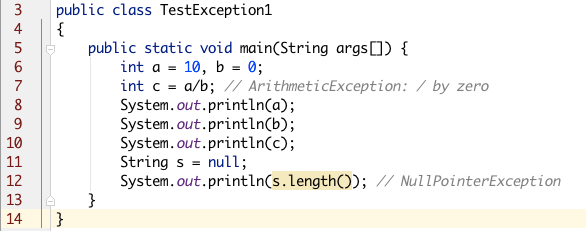
\includegraphics[width=\textwidth]{UncaughtException.png}
\end{frame}


%------------------------------------------------
\section{Caught Exceptions}
%------------------------------------------------

\begin{frame}
\frametitle{Caught Exceptions}
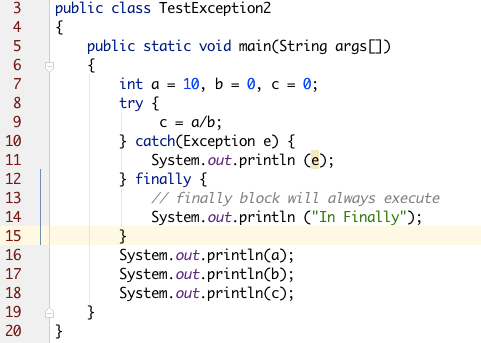
\includegraphics[width=\textwidth]{CaughtException.png}
\end{frame}


%------------------------------------------------
\section{Throws}
%------------------------------------------------

\begin{frame}
\frametitle{Throws}
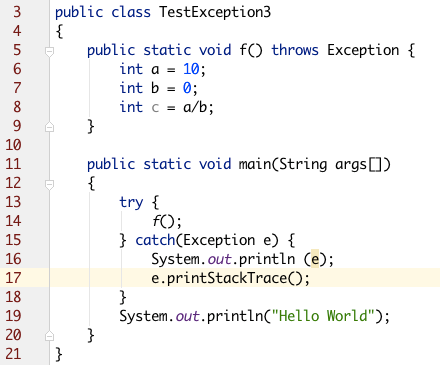
\includegraphics[width=0.9\textwidth]{Throws.png}
\end{frame}



%------------------------------------------------
\section{Custom Exceptions}
%------------------------------------------------

\begin{frame}
\frametitle{Custom Exceptions}
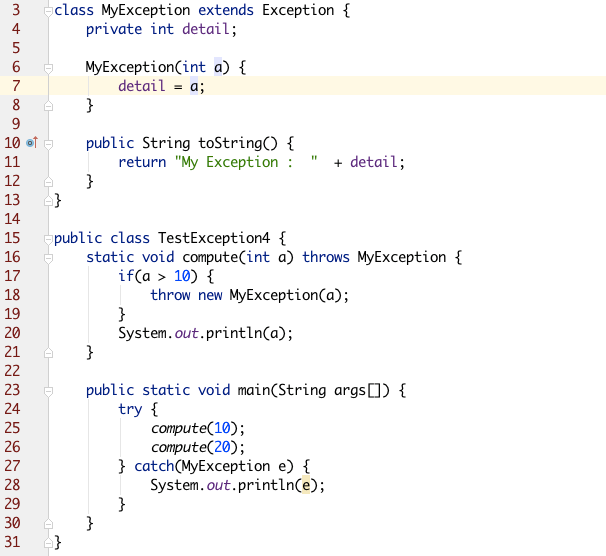
\includegraphics[width=0.85\textwidth]{CustomException.png}
\end{frame}



%-----------------------------------------------
\section{Switch}
%------------------------------------------------

\begin{frame}
\frametitle{Switch}
\end{frame}

%------------------------------------------------



%------------------------------------------------
\section{Interface}
%------------------------------------------------

\begin{frame}
\frametitle{Interface}
\end{frame}


%------------------------------------------------
\section{Abstract Class}
%------------------------------------------------

\begin{frame}
\frametitle{Abstract Class}
\end{frame}

\begin{frame}
\Huge{\centerline{THE END }}
\end{frame}

%----------------------------------------------------------------------------------------

\end{document} 